\documentclass{article}

% Bibliography
\usepackage{natbib}
\bibpunct{(}{)}{;}{a}{}{;}

% Use 'It was found that A is B (Name 1234)' style
\setcitestyle{authoryear,open={},close={}}

% Affiliations
\usepackage{authblk}
\title{babette: BEAUti 2, BEAST2 and Tracer for R}
\author[1]{Rich\`el J.C. Bilderbeek}
\author[1]{Rampal S. Etienne}
\affil[1]{Groningen Institute for Evolutionary Life Sciences, University of Groningen, Groningen, The Netherlands}

% Use double spacing
\usepackage{setspace}
\doublespacing

\usepackage{listings}
\usepackage{hyperref}
\usepackage{todonotes}
\usepackage{verbatim}
\usepackage{tikz}
\usepackage{tkz-graph}
\usepackage{pgf}
\usepackage{bm}

\usetikzlibrary{arrows,automata}

% Style of listings
% From http://r.789695.n4.nabble.com/How-to-nicely-display-R-code-with-the-LaTeX-package-listings-tp4648110.html
\usepackage{fancyvrb} 
\definecolor{codegreen}{rgb}{0,0.6,0}
\definecolor{codegray}{rgb}{0.5,0.5,0.5}
\definecolor{codepurple}{rgb}{0.58,0,0.82}
\definecolor{backcolor}{rgb}{0.95,0.95,0.92}
\lstdefinestyle{mystyle}{
  language=R,% set programming language
  basicstyle=\ttfamily\small,% basic font style
  commentstyle=\color{gray},% comment style
  % numbers=left,% display line numbers on the left side
  numberstyle=\scriptsize,% use small line numbers
  numbersep=10pt,% space between line numbers and code
  tabsize=2,% sizes of tabs
  showstringspaces=false,% do not replace spaces in strings by a certain character
  captionpos=b,% positioning of the caption below
  breaklines=true,% automatic line breaking
  escapeinside={(*}{*)},% escaping to LaTeX
  fancyvrb=true,% verbatim code is typset by listings
  extendedchars=false,% prohibit extended chars (chars of codes 128--255)
  alsoletter={.<-},% becomes a letter
  alsoother={$},% becomes other
  otherkeywords={!=, ~, $, \&, \%/\%, \%*\%, \%\%, <-, <<-, /},% other keywords
  deletekeywords={c}% remove keywords 
}
\lstset{style=mystyle}

% Adds numbered lines
\usepackage{lineno}
\linenumbers

% Rename 'Abstract' to 'Summary 
\usepackage[english]{babel}
\addto{\captionsenglish}{\renewcommand{\abstractname}{Summary}}

\usetikzlibrary{calc}
\usetikzlibrary{arrows.meta}

\begin{document}

\maketitle

\begin{abstract}

  \textbf{1. }
    In the field of phylogenetics, 
    BEAST2 is one of the most widely used software tools. 
    It comes with the graphical user interfaces BEAUti 2, DensiTree and Tracer,
    to create BEAST2 configuration files and to interpret BEAST2's output files. 
    However, when many different alignments or model 
    setups are required, a workflow of graphical user interfaces is cumbersome. \\
  \textbf{2. }
    Here, we present a free, libre and open-source package, \verb;babette;: 
    'BEAUti 2, BEAST2 and Tracer for R', for the R programming language. 
    \verb;babette; creates BEAST2 input files, runs BEAST2 and parses its results, 
    all from an R function call. \\
  \textbf{3. }
    We describe \verb;babette;'s usage and the novel functionality it provides
    compared to the original tools and we give some examples. \\
  \textbf{4. }
    As \verb;babette; is designed to be of high quality and extendable, 
    we conclude by describing the further development of the package. \\
\end{abstract}

{\bf Keywords:} computational biology, evolution, phylogenetics, BEAST2, R

%%%%%%%%%%%%%%%%%%%%%%%%%%%%%%%%%%%%%%%%%%%%%%%%%%%%%%%%%%%%%%%%%%%%%%%%%%%%%%%%%%%%%%
\section{Introduction}
%%%%%%%%%%%%%%%%%%%%%%%%%%%%%%%%%%%%%%%%%%%%%%%%%%%%%%%%%%%%%%%%%%%%%%%%%%%%%%%%%%%%%%

Phylogenies are commonly used to explore evolutionary hypotheses.
Not only can phylogenies show us how species (or other
evolutionary units) are related to each other, 
but we also estimate relevant parameters such as extinction and 
speciation rates.
There are many phylogenetics tools available to obtain an estimate 
of the phylogenetic tree of a given set of species. 
BEAST2 (\cite{bouckaert2014beast}) is one of the most widely used ones. 
It creates a posterior of jointly estimated phylogenies and model parameters, 
from one or more DNA, RNA or amino acid alignments (see figure \ref{fig:workflow} 
for an overview of the workflow). 
It has a graphical and a command-line interface, 
that both need a configuration file containing 
alignments and model parameters.
BEAST2 is bundled with BEAUti 2 (\cite{drummond2012bayesian}) ('BEAUti' from now on), 
a desktop application to create a BEAST2 configuration file.
BEAUti has a user-friendly graphical user interface, with helpful
default settings.
As such, BEAUti is an attractive alternative 
to manual and error-prone editing of BEAST2 configuration files. 

However, BEAUti cannot be called from a command-line script.
This implies that when the user 
wants to explore the consequences of various settings, this must be done manually.
This is the managable workflow when using a few alignments and doing a superficial 
analysis of sensitivity of the reconstructed tree to model settings. 
For exploring many trees (for instance from simulations) and for
more thorough sensitivity analysis, one would like to loop through 
multiple (simulated) alignments, nucleotide substitution models, 
clock models and tree priors. 
One such tool to replace BEAUti is \verb;BEASTmasteR; (\cite{beastmaster}),
which focuses on morphological traits and tip-dating, but also 
supports DNA data. \verb;BEASTmasteR;, however, requires hundreds of
lines of R code to setup the BEAST2 model configuration 
and a Microsoft Excel file to specify alignment files.

BEAST2 is also associated with Tracer (\cite{tracer}) and 
DensiTree (\cite{DensiTree}). Both are desktop applications 
to analyze the output of BEAST2, each with a user-friendly graphical user interface. 
Tracer's purpose is to analyze the parameter estimates generated
from a BEAST2 run. It shows, among
others, the effective sample size (ESS) and time series ('the trace', 
hence the name) of each variable in the MCMC run. Both ESS and trace
are needed to assess the strength of the inference. 
DensiTree visualizes the phylogenies of a BEAST2 posterior, with
many options to improve the simultaneous display of many phylogenies.

However, for exploring the output of many BEAST2 runs, 
one would like a script to collect all parameters' ESSes,
parameter traces and posterior phylogenies.
There is no single package that offers a complete solution,
but examples of R packages that offer a partial solution
are \verb;BEASTmasteR;, \verb;rBEAST; 
(\cite{rBEAST_ratmann}) and 
\verb;RBeast; (\cite{RBeast_faria}). 
\verb;BEASTmasteR; is a partial BEAUti alternative,
does not offer a way to call BEAST2, 
nor allows for the same data analysis as done by Tracer. 
\verb;RBeast; provides some plotting options and parsing
of BEAST2 output files. \verb;rBEAST; is a package developed
around testing a biological hypothesis, 
that does not aim to be a generally used package.

Here, we present \verb;babette;:
’BEAUti 2, BEAST2 and Tracer for R’, 
which creates BEAST2 (v.2.4.7) configuration files,
runs BEAST2, and analyzes its results,
all from an R function call. This
will save time, tedious mouse clicking and 
reduces the chances of errors in such repetitive actions.
The interface of \verb;babette; mimics the tools it
is based on. This
familiarity helps both beginner and experienced BEAST2 users 
to make the step from those tools to \verb;babette;.
\verb;babette; enables the creation of a single-script 
pipeline from sequence alignments to posterior analysis in R. 

%%%%%%%%%%%%%%%%%%%%%%%%%%%%%%%%%%%%%%%%%%%%%%%%%%%%%%%%%%%%%%%%%%%%%%%%%%%%%%%%%%%%%%
\section{Description}
%%%%%%%%%%%%%%%%%%%%%%%%%%%%%%%%%%%%%%%%%%%%%%%%%%%%%%%%%%%%%%%%%%%%%%%%%%%%%%%%%%%%%%

\verb;babette; is written in the R programming language (\cite{R})
and enables the full BEAST2 workflow from an R function call,
in a similar way to what BEAUti, DensiTree and Tracer do.
\verb;babette;'s main function is \verb;run_beast2;, which
configures BEAST2, runs it and parses its output. 
\verb;run_beast2; needs at least the name of a 
FASTA file containing a DNA alignment. 
The default settings for the other arguments of \verb;run_beast2; 
are identical to BEAUti's and BEAST2's default settings.
Per alignment, a site model, clock model and tree prior can be chosen.
Multiple alignments can be used, each with its own (unlinked) site model, 
clock model and tree prior.

\verb;babette; currently has 100 exported functions to set up  
a BEAST2 configuration file. 
\verb;babette; can currently handle a majority of BEAUti use cases.
Because of BEAUti's high number of plugins, 
\verb;babette; uses a software architecture that is designed to be extended.
Furthermore, \verb;babette; has 12 exported functions to run and help run BEAST2.
One function is used to run BEAST2, others
allow the user to check if a BEAST2 configuration file is indeed valid.
Finally, \verb;babette; has 21 exported function to parse the BEAST2 output
files and analyze the created posterior. \verb;babette; gives the
same ESSes and summary statistics as Tracer. The data is formatted
such that it can easily be visualized using \verb;ggplot2; (for a trace,
similar to Tracer) or \verb;phangorn; (\cite{phangorn}) (for 
the phylogenies in a posterior, similar to DensiTree). 

Currently, \verb;babette; does not replace all functionality in BEAUti,
as it does not provide 3 out of 7 tree priors, nor does it support RNA
alignments or use of morphological data. The many plug-ins of BEAUti
are not yet supported by \verb;babette;. \verb;babette; does not support
all command-line arguments of BEAST2, does not provide
the more specialized Tracer analysis options, nor is it as feature-rich
in plotting options as DensiTree. Up until now, the \verb;babette; features 
implemented are those requested by users. Further extension of \verb;babette; 
will be based on future user requests.

%%%%%%%%%%%%%%%%%%%%%%%%%%%%%%%%%%%%%%%%%%%%%%%%%%%%%%%%%%%%%%%%%%%%%%%%%%%%%%%%%%%%%%
\section{Usage}
%%%%%%%%%%%%%%%%%%%%%%%%%%%%%%%%%%%%%%%%%%%%%%%%%%%%%%%%%%%%%%%%%%%%%%%%%%%%%%%%%%%%%%

In R, the functions of a package need to be loaded in the global namespace first:

\begin{lstlisting}[language=R, floatplacement=H]
library(babette)
\end{lstlisting}
BEAUti, and likewise \verb;babette;, needs at least a FASTA filename
to produce a BEAST2 configuration file. 
In BEAUti, this is achieved by loading a FASTA file, 
then saving an output file using a common
save file dialog. After this, BEAST2 needs to be applied to
the created configuration file. It creates multiple files
storing the posterior. These output
files must be parsed by either Tracer of DensiTree.
In \verb;babette;, all this is achieved by:

\begin{lstlisting}[language=R, floatplacement=H]
out <- run_beast2("anthus_aco.fas")
\end{lstlisting}
This code will create a (temporary) BEAST2 configuration file,
from the FASTA file with name \verb;anthus_aco.fas; (which
is supplied with the package, from (\cite{VanEls2018})), 
using the same default settings as BEAUti, which are, 
among others, a Jukes-Cantor site model, a strict clock, and a Yule birth tree prior.
\verb;babette; will then execute BEAST2 using that file, and
parses the output. The returned data structure, named \verb;out;, 
is a list of parameter estimates (called \verb;estimates;), posterior 
phylogenies (called \verb;anthus_aco_trees;, named after
the alignment's name) and MCMC operator performance (\verb;operators;).
An example of using a different site model, clock model 
and tree prior is:

\begin{lstlisting}[language=R, floatplacement=H]
out <- run_beast2(
  "anthus_aco.fas",
  site_models = create_hky_site_model(),
  clock_models = create_rln_clock_model(),
  tree_priors = create_bd_tree_prior()
)
\end{lstlisting}
This code uses an HKY site model, a relaxed log-normal clock model and a 
birth-death tree prior, each with their default settings in BEAUti.
Table \ref{tab:functions} shows an overview of all functions to 
create site models, clock models and tree priors.
Note that the arguments' names \verb;site_models;, \verb;clock_models; 
and \verb;tree_priors; are plural, as each of these
can be (a list of) one or more elements. Each of these arguments must 
have the same number of elements, so that each alignment has its
own site model, clock model and tree prior. 
An example of two alignments, each with its own site model, is:

\begin{lstlisting}[language=R, floatplacement=H]
out <- run_beast2(
  c("anthus_aco.fas", "anthus_nd2.fas"),
  site_models = list(
    create_tn93_site_model(), 
    create_gtr_site_model()
  )
)
\end{lstlisting}
\verb;babette; also uses the same default prior distributions as BEAUti 
for each of the site models, clock models and tree priors. 
For example, by default, a Yule tree prior assumes that the birth rate 
follows a uniform distribution, 
from minus infinity to plus infinity. 
This assumption implies that negative and positive birth rates are just as likely, 
where a negative birth rate is biologically impossible (note that 
in practice, this usually works out just fine).
One may prefer an exponential distribution instead, 
as this would assume only positive birth rates, 
and makes high birth rates unlikely.
To do this in \verb;babette;:

\begin{lstlisting}[language=R, floatplacement=H]
out <- run_beast2(
  "anthus_aco.fas",
  tree_priors = create_yule_tree_prior(
    birth_rate_distr = create_exp_distr()    
  )
)
\end{lstlisting}
In this same example, one may specify
the initial shape parameters of the exponential distribution.
In BEAST2's implementation, an exponential distribution 
has one shape parameter: its mean, which can be set to any
value with \verb;BEAUti;. Within \verb;babette;, to set the 
mean value of the exponential distribution to a 
fixed (non-estimated) value, do: 

\begin{lstlisting}[language=R, floatplacement=H]
out <- run_beast2(
  "anthus_aco.fas",
  tree_priors = create_yule_tree_prior(
    birth_rate_distr = create_exp_distr(
      mean = create_mean_param(
        value = 1.0, 
        estimate = FALSE
      )
    )    
  )
)
\end{lstlisting}
Our initial motivation to create \verb;babette; 
was that we wanted to fix the crown age of a phylogeny.
BEAUti assumes that a phylogeny has a crown age that needs to be 
jointly estimated with the phylogeny and other parameters. 
It does not allow for fixing
the crown age. Without \verb;babette;, one needs to manually edit the BEAST2 
configuration file (\cite{fix_starting_tree}), which is tedious and prone to errors. 
Fixing the crown ages is especially useful for theoretical experiments,
as this allows for one less source of variation.
This is how to specify a fixed crown age with \verb;babette;:

\begin{lstlisting}[language=R, floatplacement=H]
out <- run_beast2(
  "anthus_aco.fas",
  posterior_crown_age = 15
)
\end{lstlisting}
\verb;babette; allows for the same functionality as Tracer.
Tracer works on the values of the parameter estimates sampled
in the BEAST2 run. This is called the "trace" (hence the name).
The start of the trace is usually discarded, as an MCMC 
algorithm (such as used by BEAST2) first has to converge to
its equilibrium. The start of the trace, called the "burn-in", 
will be removed, because its parameter estimates are not 
representative. By default, Tracer discards the first 10\% of all 
the parameter estimates. 
To remove a 20\% burn-in from all parameter estimates 
in \verb;babette;, the following code can be used:

\begin{lstlisting}[language=R, floatplacement=H]
traces <- remove_burn_ins(
  out$estimates, 
  burn_in_fraction = 0.2
)
\end{lstlisting}
Tracer shows the ESSes of each posterior's variables.
These ESSes are important to determine the strength of the
inference. As a rule of thumb, an ESS of 200 is acceptable 
for any parameter estimate.
To calculate the effective sample sizes (of all estimated variables) in \verb;babette;:

\begin{lstlisting}[language=R, floatplacement=H]
esses <- calc_esses(
  traces, 
  sample_interval = 1000
)
\end{lstlisting}
Tracer displays multiple summary statistics for each
estimated variable: the mean and its standard error, standard deviation,
variance, median, mode, geometric mean, 95\% highest posterior density interval, 
auto-correlation time and effective sample size. It displays these statistics per
variable. In \verb;babette;, these summary statistics are collected for
all estimated parameters at once: 

\begin{lstlisting}[language=R, floatplacement=H]
sum_stats <- calc_summary_stats(
  traces, 
  sample_interval = 1000
)
\end{lstlisting}
\verb;babette; allows for the same functionality as DensiTree.
DensiTree displays the phylogenies in a posterior at the same
time scale, drawn one over one another, allowing to see the uncertainty in
topology and branch lengths. Within the object \verb;out;, 
the posterior phylogenies are stored as \verb;anthus_aco_trees;,
and can be plotted as such:

\begin{lstlisting}[language=R, floatplacement=H]
plot_densitree(out$anthus_aco_trees)
\end{lstlisting}

%%%%%%%%%%%%%%%%%%%%%%%%%%%%%%%%%%%%%%%%%%%%%%%%%%%%%%%%%%%%%%%%%%%%%%%%%%%%%%%%%%%%%%
\section{babette resources}
%%%%%%%%%%%%%%%%%%%%%%%%%%%%%%%%%%%%%%%%%%%%%%%%%%%%%%%%%%%%%%%%%%%%%%%%%%%%%%%%%%%%%%

\verb;babette; is free, libre and open source software available 
from the official R package archive at 
\url{http://cran.r-project.org/src/contrib/PACKAGES.html\#babette}
and is licensed under the GNU General Public License v3.0.
\verb;babette; uses the Travis CI (\url{https://travis-ci.org})
continuous integration service, which is known to significantly 
increase the number of bugs exposed (\cite{vasilescu2015}) and increases
the speed at which new features are added (\cite{vasilescu2015}).
\verb;babette; has a 100\% code coverage, which correlates with 
code quality (\cite{horgan1994,del1995correlation}). 
\verb;babette; follows Hadley Wickham's style guide (\cite{style_guide}), 
which improves software quality (\cite{fang2001}).
\verb;babette; dependends on multiple packages, which are 
\verb;ape; (\cite{APE}), 
\verb;beautier; (\cite{beautier}),
\verb;beastier; (\cite{beastier}),
\verb;devtools; (\cite{devtools}),
\verb;geiger; (\cite{GEIGER}),
\verb;ggplot2; (\cite{ggplot2}),
\verb;knitr; (\cite{knitr}),
\verb;phangorn; (\cite{phangorn}),
\verb;rmarkdown; (\cite{rmarkdown}),
\verb;seqinr; (\cite{seqinr}),
\verb;stringr; (\cite{stringr}),
\verb;testit; (\cite{testit}) and 
\verb;tracerer; (\cite{tracerer}).
\verb;babette; is tested to give a clean 
error message for incorrect input, by
calling \verb;babette; one million times
with random or random sensible inputs, 
using the Peregrine high performance computer cluster. 
The scripts to do so, are supplied with \verb;babette;.

\verb;babette;'s development takes place on GitHub,
\url{https://github.com/richelbilderbeek/babette}, 
which accommodates collaboration (\cite{perez2016ten}) 
and improves transparency (\cite{gorgolewski2016practical}).
\verb;babette;'s GitHub facilitates feature requests and 
has guidelines how to do so.

\verb;babette;'s documentation is extensive. All functions are documented
in the package's internal documentation. For quick use, 
each exported function shows a minimal example. 
For easy exploration, each exported function's documentation links to related functions.
Additionally, \verb;babette; has a vignette that demonstrates extensively how
to use it. There is documentation on the GitHub to get started, 
with a dozen examples of BEAUti screenshots with equivalent \verb;babette; code.
Finally, \verb;babette; has some tutorial video's that can 
be downloaded or viewed on YouTube, \url{https://goo.gl/weKaaU}.

%%%%%%%%%%%%%%%%%%%%%%%%%%%%%%%%%%%%%%%%%%%%%%%%%%%%%%%%%%%%%%%%%%%%%%%%%%%%%%%%%%%%%%
\section{Citation of babette}
%%%%%%%%%%%%%%%%%%%%%%%%%%%%%%%%%%%%%%%%%%%%%%%%%%%%%%%%%%%%%%%%%%%%%%%%%%%%%%%%%%%%%%

Scientists using \verb;babette; in a published paper can cite this
article, and/or cite the \verb;babette; package 
directly. To obtain this citation from within an R script, use:

\begin{lstlisting}[language=R]
> citation("babette")
\end{lstlisting}

%%%%%%%%%%%%%%%%%%%%%%%%%%%%%%%%%%%%%%%%%%%%%%%%%%%%%%%%%%%%%%%%%%%%%%%%%%%%%%%%%%%%%%
\section{Acknowledgements}
%%%%%%%%%%%%%%%%%%%%%%%%%%%%%%%%%%%%%%%%%%%%%%%%%%%%%%%%%%%%%%%%%%%%%%%%%%%%%%%%%%%%%%

Thanks to Yacine Ben Chehida and Paul van Els for supplying their 
BEAST2 use cases. Thanks again to Paul van Els for the sharing his FASTA files 
for use by this package. Thanks to Leonel Herrera-Alsina, Raphael Scherrer 
and Giovanni Laudanno for their comments on this package and article.
We would like to thank the Center for Information Technology of the University 
of Groningen for their support and for providing access to the Peregrine 
high performance computing cluster.

%%%%%%%%%%%%%%%%%%%%%%%%%%%%%%%%%%%%%%%%%%%%%%%%%%%%%%%%%%%%%%%%%%%%%%%%%%%%%%%%%%%%%%
% Bibliography
%%%%%%%%%%%%%%%%%%%%%%%%%%%%%%%%%%%%%%%%%%%%%%%%%%%%%%%%%%%%%%%%%%%%%%%%%%%%%%%%%%%%%%
% MEE style
\bibliographystyle{mee}
\bibliography{article}
%%%%%%%%%%%%%%%%%%%%%%%%%%%%%%%%%%%%%%%%%%%%%%%%%%%%%%%%%%%%%%%%%%%%%%%%%%%%%%%%%%%%%%




%%%%%%%%%%%%%%%%%%%%%%%%%%%%%%%%%%%%%%%%%%%%%%%%%%%%%%%%%%%%%%%%%%%%%%%%%%%%%%%%%%%%%%
% Figures at the end
%%%%%%%%%%%%%%%%%%%%%%%%%%%%%%%%%%%%%%%%%%%%%%%%%%%%%%%%%%%%%%%%%%%%%%%%%%%%%%%%
\begin{figure}
  \centering
  \resizebox {0.8\columnwidth} {!} {
    \begin{tikzpicture}[->,>=stealth',shorten >=1pt,auto,node distance=6cm, semithick]   
    \tikzstyle{every state}=[]
    \node[state] (A) [rectangle] {
      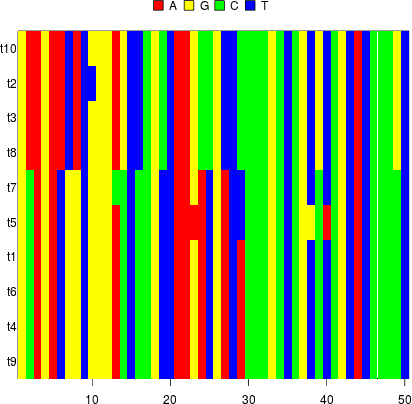
\includegraphics[width=0.2\textwidth]{alignment.png}
    };   
    \node[state] (AL) [above left=-0.25cm and -0.25cm of A, fill=white] {
      1
    };   
    \node[state] (B) [right of = A, rectangle] {
      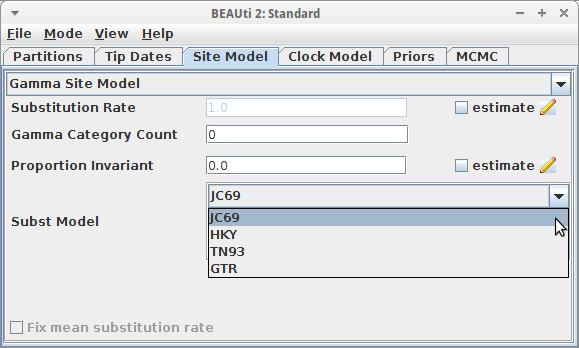
\includegraphics[height=0.15\textheight]{BeautiSiteModel.png}
    };   
    \node[state] (BL) [above left=-0.25cm and -0.25cm of B, fill=white] {
      2
    };   
    \node[state] (E) [below of=A, rectangle] {
      
\includegraphics[height=0.1\textheight]{file2.png}
    };   
    \node[state] (EL) [above left=-0.25cm and -0.25cm of E, fill=white] {
      3
    };   
    \node[state] (C) [right of = E, rectangle] {
      
\includegraphics[width=0.3\textwidth]{beast_logo.png}
    };   
    \node[state] (CL) [above left=-0.25cm and -0.25cm of C, fill=white] {
      4
    };   
    \node[state] (F) [rectangle, below of=E] {
      
\includegraphics[height=0.1\textheight]{file.png}
    };
    \node[state] (FL) [above left=-0.25cm and -0.25cm of F, fill=white] {
      5
    };   
    \node[state] (H) [rectangle, below of=F] {
      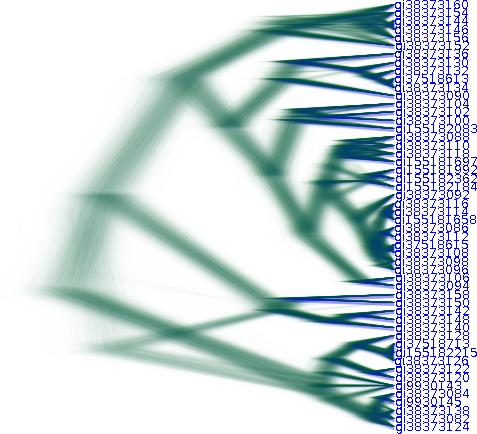
\includegraphics[width=0.3\textwidth]{DensiTreeExample2.jpg}
    };
    \node[state] (HL) [above left=-0.25cm and -0.25cm of H, fill=white] {
      6
    };   
    \node[state] (I) [rectangle, right of=H] {
      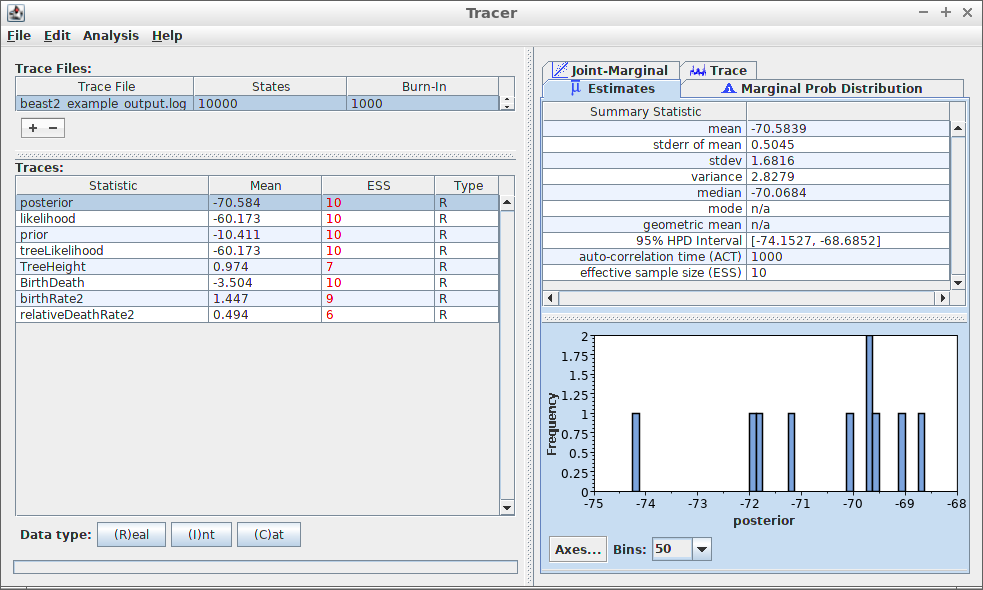
\includegraphics[width=0.6\textwidth]{tracer_example_output.png}
    };
    \node[state] (IL) [above left=-0.25cm and -0.25cm of I, fill=white] {
      7
    };   
    \path 
      (A) edge [anchor = west] node {} (E)
      (E) edge [anchor = west] node {} (F)
      (F) edge [anchor = west] node {} (H)
      (F) edge [anchor = west] node {} (I)
    ; 
    \path [-o,draw] (B) -- ($ (A) !.5! (E) $);
    \path [-o,draw] (C) -- ($ (E) !.5! (F) $);
    \end{tikzpicture}
  }
  \caption{
    Workflow using GUI tools. From an alignment (1) and BEAUti (2), 
    a BEAST2 configuration file (3) is created. BEAST2 (4) uses that file
    to infer a posterior, storing it in multiple files (5). These results
    are visualized using DensiTree (6) and Tracer (7). babette allows
    for the same workflow, all from an R function call.
  }
  \label{fig:workflow}
\end{figure}
%%%%%%%%%%%%%%%%%%%%%%%%%%%%%%%%%%%%%%%%%%%%%%%%%%%%%%%%%%%%%%%%%%%%%%%%%%%%%%%%

%%%%%%%%%%%%%%%%%%%%%%%%%%%%%%%%%%%%%%%%%%%%%%%%%%%%%%%%%%%%%%%%%%%%%%%%%%%%%%%%%%%%%%
\begin{table}[h]
\centering
\begin{tabular}{ | l | l | }
\hline
\textbf{Name} & \textbf{Description} \\
\hline
\verb;run_beast2; & Run BEAST2 \\
\hline
\verb;create_gtr_site_model; & Create a GTR site model \\
\verb;create_hky_site_model; & Create an HKY site model \\
\verb;create_jc69_site_model; & Create a Jukes-Cantor site model \\
\verb;create_tn93_site_model; & Create a TN93 site model \\
\hline
\verb;create_rln_clock_model; & Create a relaxed log-normal clock model \\
\verb;create_strict_clock_model; & Create a strict clock model \\
\hline
\verb;create_bd_tree_prior; & Create a birth-death tree prior \\
\verb;create_cbs_tree_prior; & Create a coalescent Bayesian skyline tree prior \\
\verb;create_ccp_tree_prior; & Create a coalescent constant-population tree prior \\
\verb;create_cep_tree_prior; & Create a coalescent exponential-population tree prior \\
\verb;create_yule_tree_prior; & Create a Yule tree prior \\
\hline
\verb;create_beta_distr; & Create a beta distribution \\
\verb;create_exp_distr; & Create an exponential distribution \\
\verb;create_gamma_distr; & Create a gamma distribution \\
\verb;create_inv_gamma_distr; & Create an inverse gamma distribution \\
\verb;create_laplace_distr; & Create a Laplace distribution \\
\verb;create_log_normal_distr; & Create a log-normal distribution \\
\verb;create_normal_distr; & Create a normal distribution \\
\verb;create_one_div_x_distr; & Create a 1/X distribution \\
\verb;create_poisson_distr; & Create a Poisson distribution \\
\verb;create_uniform_distr; & Create a uniform distribution \\
\hline
\end{tabular}
\caption{babette's main functions}
\label{tab:functions}
\end{table}
%%%%%%%%%%%%%%%%%%%%%%%%%%%%%%%%%%%%%%%%%%%%%%%%%%%%%%%%%%%%%%%%%%%%%%%%%%%%%%%%%%%%%%

\end{document}
\grid
\grid
\grid
\grid
